% \vspace{-0.2\baselineskip}
\section{Evaluation}
% \vspace{-0.3\baselineskip}
\label{sec:evaluation}
In this section, the datasets and evaluation metrics are firstly introduced. We then describe the implementation details of the framework. Compreshensive experiments have been conducted to validate the effectiveness of our approach on different setups of the object detection task.

\subsection{Datasets and metrics}
We conducted experiments on object detection task using different types of setup. The performances are evaluated on two datasets: (1) the Charades dataset \cite{sigurdsson2016hollywood}, which consists of daily-life videos captured by hand-held devices and (2) HICO-DET dataset, which contains images of various human-object interactions.
Two different object detection metrics are used during evaluation.

\textbf{Datasets.} As introduced in Sec. \ref{sec:intro}, the activity driven weakly supervised detection task takes video or images and corresponding action label as training samples, and is evaluated on static images, where object bounding boxes are annotated. We select a video dataset (Charades) and an image dataset (HICO-DET) for evaluation.

 The Charades dataset includes 9,848 videos of 157 action classes, among which, 66 are interactive actions with objects. There are on average 6.8 action labels for one video, resulting in a total of 67,000 clips. The official Charades dataset doesn't provide object bounding box annotations and we use the annotations released by \cite{yuan2017temporal}. 
he released annotations, 17 objects in the 66 interactive actions are labeled with bounding boxes in the test set videos. The 1,812 test videos are downsampled to 1 frame per second (fps) and then annotated on each frames. There are 3.4 bounding box annotations per frame on average. Although all downsampled frames in test set have been annotated, 5,000 frames from 200 test videos are actually used for evaluation. We follow the same practice as in \cite{yuan2017temporal}: training on the 7,986 videos (54,000 clips) in training set and evaluate on 5,000 test frames to directly compare with the current SOTA methods.

The HICO-DET dataset is designed for the human-object interaction (HOI) task, which includes 38,118 training images and 9,658 test images. The human bounding box, object bounding box and an HOI class label are annotated for both training and test images. In total, there are 80 object classes (\eg~\textit{cup}, \textit{dog}, \etc) and 600 HOI classes (\eg~\textit{hold cup}, \textit{feed dog}, \etc) annotated. We use the HOI labels as action class labels during training and the object bounding box annotations are used during evaluation. Different from Charades where the interactions often happen between one subject and one object, there are cases multiple people interacting with one object (\eg~``boarding the airplane'') and one people interacting with multiple objects (\eg~``herding cows''), which makes it more challenging to learn the object appearance.

\textbf{Evaluation metrics.} We have conducted experiments to evaluate the object detection performances on the test set of the two datasets. We report per-class \textit{average precision} (AP) at \textit{intersection-over-union} (IoU) of 0.5 between detection and ground truth boxes, and also mean AP (mAP) as a combined metric, following the tradition of \cite{yuan2017temporal}. The evaluation toolbox released by \cite{girshick2015fast} is slightly modified to adapt to Charades dataset. We also report \textit{CorLoc} \cite{deselaers2012weakly}, a commonly-used weakly supervised detection metric. CorLoc represents the percentage of images where at least one instance of the target object class is correctly detected (IoU\textgreater0.5) over all images that contain at least one instance of the class. The evaluation code in TensorFlow detection metric toolkit is directly used.

\subsection{Implementation details}
We adopt a pre-trained convolutional neural network as our backbone feature extraction network ($\phi()$). For comparison between different network architectures, we experimented with VGG-16 and ResNet-101 architectures, pretrained on ImageNet dataset. All \textit{conv} layers in the network are followed with \textit{ReLU} activation except for the top layer. Batch normalization \cite{ioffe2015batch} is performed on all convolutional layers. We replace the \textit{fc} layer following the last convolutional block to classify person region and object proposals. In practice, we use three sibling classification layers. One of them is used for person region action classification, classifying the person region feature to a 66-dimensional score. The other two are used for classifying object proposals to action classes (66-dimensional scores) and object classes (18-dimensional scores) respectively.

The attention module includes action-keypoint mapping and the location probability mapping. To select the dominant keypoint given an action class, we model the mapping with a 2D matrix with size $n_a\times n_{kp}$. Numbers in the matrix represent the importance of one keypoint for an action class. For given action class, the top keypoint is selected after applying softmax on the importance weights. During training, the selected keypoint location is involved in the attention weight calculation $f_{\mu, \sigma}(r_k)$, thus the action-keypoint mapping matrix can be back-propagated and updated. The attention for object location probability is modeled with a action and time step dependent 2D spatial normal distribution. The parameters include distribution mean $\mu \in \mathbbm{R}^{n_a\times\scr{K}\times2}$, and variance $\sigma \in \mathbbm{R}^{n_a\times\scr{K}\times2\times2}$.

Object classification loss for each proposal is weighted by the distribution weight calculated from the proposal location and the weighted sum is used as object classification loss. The action classification score for each proposal is also weighted with the distribution probability and added to the action classification score from the person bounding box. The binary cross entropy loss is calculated between the combined score and ground truth action class.

In our implementation, the Adam optimizer \cite{kingma2014adam} is implemented with $\beta_1=0.9$, $\beta_2=0.999$, learning rate of $2\times 10^{-5}$ and batch size of $4$. The balance between the two loss terms is adjusted thus they have similar value scales and the hyperparameters $w_a$, $w_o$ are validated on a held-out validation set. In practice, the loss weights are set as $w_a=1.0$, $w_o=2.0$. The mean and variance matrix $\mu$, $\sigma$ are initialized as $\mathbbm{0}$ and diagonal matrix $diag(10)$. The input frames are resized such that the shorter side is 600 pixels, following the same practice in 
\cite{ren2015faster}. The number of sampled frames in a clip is set as $\scr{K}=8$ and the number of proposals per frame is set as $n_R=700$. The whole framework is implemented with PyTorch framework. On a single Nvidia Tesla M40 GPU, 11GB of memory is occupied with batch size of 4. It takes around 20 hrs to converge on a single card. The inference time for a VGA-size input image is around 0.10s.

\subsection{Experiment setup}
The weakly supervised object detection is evaluated on both Charades and HICO-DET datasets. For Charades dataset, 8 frames are uniformly sampled from each temporally trimmed training clips, resulting in 54,000 training samples. There are 47,605 test frames annotated with object bounding boxes in the release by \cite{yuan2017temporal}. Following the practice in \cite{yuan2017temporal}, we use 5,000 frames for test and the rest for training in our semi-supervision setup (details are presented in Sec. \ref{sec:supervision}). To filter out noisy object proposals and to leverage the object location temporal consistency, a linking step as in \cite{gkioxari2015finding} is applied on object proposals to form a tubelet across the 8 sampled frames. For HICO-DET dataset, training set exclusing all ``no\_interaction'' labels and interaction class with less than 20 samples are used during training, resulting in 32,100 training samples of 520 interaction classes and 80 object classes. During training, the interaction class label is used as action classification label and the object annotation bounding boxes are only used in the semi-supervision setup. During test, the object bounding box annotations on test set (9658 images) are used.

To better understand the effectivenss of each module in our approach, we conducted comprehensive ablation study experiments on Charades dataset. On both Charades and HICO-DET datasets, different weakly supervised and semi-supervised training setups are evaluated. We also compared current SOTA methods and other baseline methods we proposed on these two datasets. As there is limited number of works which report object detection performance on these two datasets, we constructed our own baseline methods by incorporating person detection and pose estimation into other SOTA methods \cite{gkioxari2015finding,bilen2016weakly}. 

\subsection{Ablation study}
To explore how much each module contributes to the final performance, we investigate with different variants of our framework: different backbone architecture, different attention modules and different loss term combinations. The backbone architectures include VGG-16 and ResNet-101. The different attention modules include distribution and grid based attention mechanism. We make a discrete version of attention module by predefining a $3\times 3$ grid around the keypoint, and the size of each cell of the grid is fixed to be $64\times 64$. There is an estimated weight for each cell as attention and all proposals whose centers fall into the cell will be assigned with the attention weight. A comparison of learned distribution and grid attention weight is shown in \figref{}. We also totally removed person detection bounding box and pose estimation from our pipeline to explore how much the person detection and pose estimation helps in object localization.
We experimented with different learning strategies for distribution attention: learning distribution mean only ($\mu$), learning variance only ($\sigma$) and joinly learning mean and variance ($\mu+\sigma$). The supervision of the proposed pipeline comes in two aspects: object classification and action classification. We experimented with applying either one supervision signal or applying both supervisions. 

\begin{table}[]
\fontsize{8}{9}\selectfont
% \def\arraystretch{1.5}
\setlength{\tabcolsep}{3pt}
\centering
\caption{Object detection performances of different variants of our approach}
\label{tbl:ab_study}
\begin{tabular}{l|c|c|c}
\specialrule{.2em}{.1em}{.1em}
Backbone  & Attention method  & Loss module  & mAP (det)    \\ \hline
VGG-16    & Distribution              & action  & 2.61   \\
VGG-16    & Distribution              & object  & 4.86   \\
VGG-16    & Distribution              & action+object  &  \textbf{6.97}   \\ \hline
VGG-16 & Distribution ($\mu$)     & action+object  & 5.46 \\ 
VGG-16 & Distribution ($\sigma$)     & action+object  & 3.27 \\
VGG-16 & Distribution ($\mu + \sigma$)    & action+object  & 6.41 \\
VGG-16 & Distribution ($\mu + \sigma, kp$ )    & action+object  & \textbf{6.87} \\\hline
VGG-16    & Grid              & action+object  & 5.41   \\
VGG-16    & Distribution      & action+object  & 6.87 \\
ResNet-101 & Grid             & action+object  & 5.59 \\
ResNet-101 & Distribution     & action+object  & \textbf{7.11} \\\hline
VGG-16    & Grid              & action  & 1.36   \\
VGG-16    & Grid              & object  & 2.67   \\
ResNet-101 & Distribution     & action  & 2.26 \\
ResNet-101 & Distribution     & object  & 3.43 \\
ResNet-101 & Distribution ($\mu$)     & action+object  & 5.46 \\ 
ResNet-101 & Distribution ($\sigma$)     & action+object  & 5.46 \\
ResNet-101 & Distribution ($\mu + \sigma$)    & action+object  & \textbf{7.11} \\\hline
\end{tabular}
\end{table}

As the quantitative results show in \tabref{tbl:ab_study}, the distribution based attention outperforms by a large margin, proving the effectiveness of learning the continuous attention weights. Another observation is from the comparison between learning $\mu$, $\sigma$ and $\mu+\sigma$ that learning all hyper-parameters in the distribution generates better performance, showing that our modeling of spatial correlation can be optimized by learning.  We encourage the object classification module to learn the object appearance and use the action classification module to help find the the most informative locations in the frame. The joint learning of both classification losses should give better performance, aligning with the numbers in \tabref{tbl:ab_study}. The qualitative results of learned object location probability are shown in Fig. \ref{fig:distribution}.

\begin{figure}
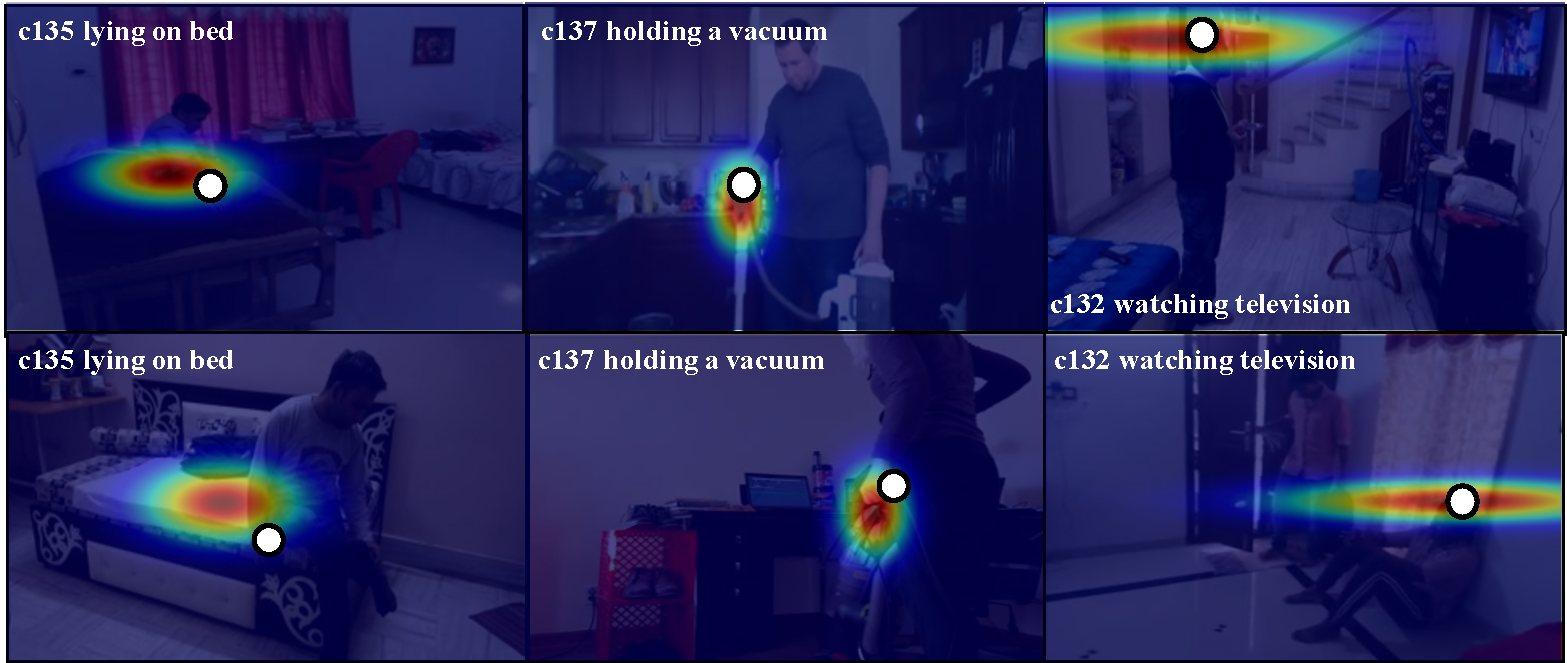
\includegraphics[width=0.5\textwidth]{figures/distribution.pdf}
% \caption{Visual comparison of depth and normal results between \protect\cite{zhou2017unsupervised} and ours. As the original depth ground truth map comes from sparse laser measurement, the interpolated depth map is shown for better visualization. As can be seen from the depth estimation, our results preserve the small/thin structures which have similar color to other foregrounds (green circles). From the normal comparison, our results predict the road normal direction better and have no artifact. The edges in normal map are also preserved better in our results (yello circles).}
\caption{Visualization of learned object location probability w.r.t. selected person keypoint. The heatmap represents the probability of object location and the white circle represents the selected keypoint.}
\label{fig:distribution}
\end{figure} 

\subsection{Supervision in training}
\label{sec:supervision}
Different training setups are explored in our experiments to explore how the pipeline benefits from incorporating ground truth information. We explored gradually adding ground truth object bounding box annotations into our supervision. Besides the object classification loss and action classification loss described in Sec. \ref{sec:approach}, an additional supervised object classification loss is added into supervision. In practice, the IoU between object proposals and ground truth object bounding boxes is calculated and proposals having higher IoU than the threshold are considered positive samples and vice versa. The threshold IoU is set as 0.45 to guarantee a reasonable positive samples per image. The negative and positive sample ratio is set as 5. 

We compare with two baseline methods: (1) a fully supervised variant of our approach: our method without pose estimation and action classification stream. Basically, only the object classification stream in Fig. \ref{fig:pipeline} is preserved; (2) R*CNN \cite{gkioxari2015contextual} with object bounding supervision. For this baseline, we incorporate object classification loss as described above into the R*CNN pipeline. The supervision comes from a combination of both object classification and action classification loss. The performance of the supervised version of our approach is shown in \tabref{tbl:sota}.

\begin{figure}
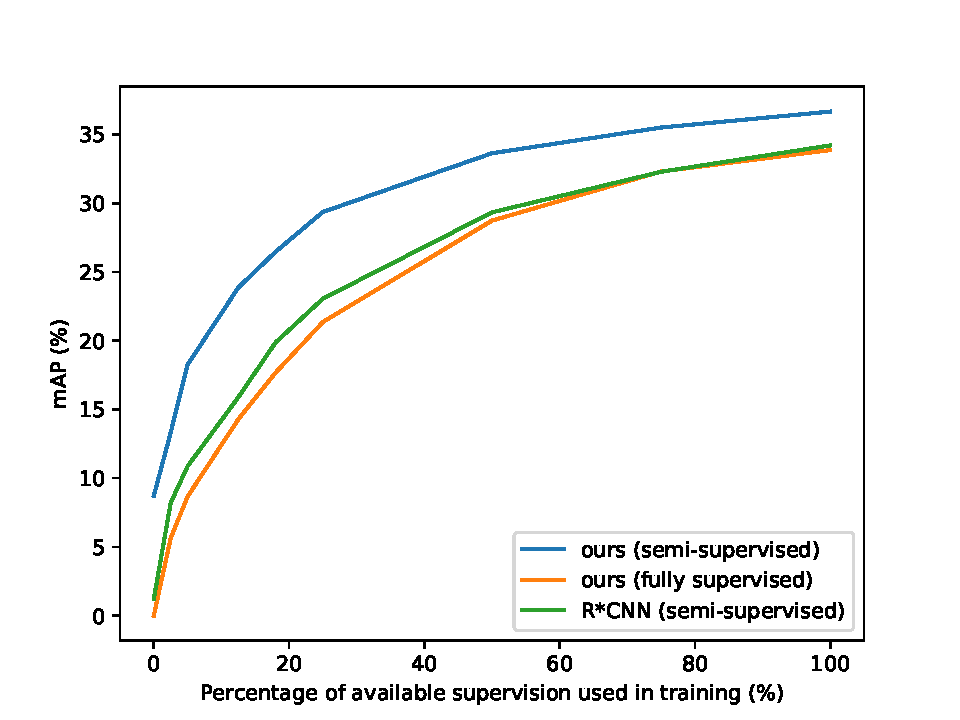
\includegraphics[width=0.5\textwidth]{figures/ratio_exp.pdf}
% \caption{Visual comparison of depth and normal results between \protect\cite{zhou2017unsupervised} and ours. As the original depth ground truth map comes from sparse laser measurement, the interpolated depth map is shown for better visualization. As can be seen from the depth estimation, our results preserve the small/thin structures which have similar color to other foregrounds (green circles). From the normal comparison, our results predict the road normal direction better and have no artifact. The edges in normal map are also preserved better in our results (yello circles).}
\caption{Performance comparison between our method trained in a semi-supervised method, fully supervised method and R*CNN trained in a semi-supervised approach.}
\label{fig:semi-supervision}
\end{figure} 

The semi-supervised training setup is evaluated on both Charades and HICO-DET datasets by incorporating partial supervision into training. The quantitative results are presented in Fig. \ref{fig:semi-supervision}. The x-axis in the two figures represents the percentage of available training samples used in training. For example, the point ``0\%'' represents that only training samples with action class labels are used and ``100\%'' means all available object bounding box annotations are used besides the weakly supervision from action class. Notice that at ``0\%'', weakly supervised method (ours and R*CNN) outperforms the fully supervised baseline as these two methods can still learn the object representation without explicit object labels. 

\begin{table*}[]
\centering
\fontsize{7.5}{8}\selectfont
\caption{AP performance (\%) on each object class and mAP (\%) comparison with different weakly supervised methods.}
\label{tbl:class_wise_charades}
\def\arraystretch{1.2}
\setlength{\tabcolsep}{3pt}
\begin{tabular}{l|ccccccccccccccccc|c}
\specialrule{.2em}{.1em}{.1em}
Methods                                        & bed & broom & chair & cup & dish & door & laptop & mirror & pillow & refri & shelf & sofa    & table   & tv   & towel       & vacuum    & window     & mAP(\%)      \\ \hline
WSDDN \cite{bilen2016weakly}                   & 2.38 & 0.04 &1.17 &0.03 & 0.13 & 0.31 & 2.81 & 0.28 & 0.02 & 0.12 & 0.03 & 0.41 & 1.74 & 1.18 & 0.07 & 0.08 & 0.22 & 0.65   \\
R*CNN \cite{gkioxari2015contextual}           & 1.87 & 0.04 & 1.73 & 0.05 & 0.08 & 0.57 & 2.75 & 0.32 & 0.10 & 0.73 & 1.04 & 1.21 & 0.55 & 1.03 & 0.07 & 0.53 & 0.32 & 0.98 \\
ContextLocNet \cite{kantorov2016contextlocnet} & 7.40 & 0.03 & 0.55 & 0.02 & 0.01 & 0.17 & 1.11 &0.66 & 0 & 0.07 & 1.75 & 4.12 & 0.63 & 0.99 & 0.03 & 0.75 & 0.78 & 1.12  \\
TD-LSTM \cite{yuan2017temporal}                & 9.19 & 0.04 & 4.18 & 0.49 & 0.11 & 1.17 & 2.91 & 0.30 & 0.08 & 0.29 & 3.21 & 5.86 & 3.35 & 1.27 & 0.09 & 0.60 & 0.47 & 1.98 \\ \hline
Ours (vgg-16)                                  & 13.82 & 8.23 & 11.38 & 6.85 & 4.21 & 5.04 & 8.31 & 4.24 & 7.34 & 14.29 & 5.37 & 15.21 & 8.46 & 2.37 & 4.06 & 6.53 & 3.07 & 8.72\\ 
Ours (ResNet-101)                              & \textbf{15.04} & \textbf{9.17} & \textbf{12.36} & \textbf{7.52} & \textbf{6.14} & \textbf{6.22} & \textbf{9.69} & \textbf{5.79} & \textbf{8.06} & \textbf{14.97} & \textbf{6.94} & \textbf{16.38} & \textbf{9.43} & \textbf{3.75} & \textbf{4.83} & \textbf{8.08} & \textbf{4.12} & \textbf{10.03}\\\hline
\end{tabular}
\end{table*}


\subsection{Comparison with SOTA}
Our method is compared with current SOTA methods as well as several baseline methods we came up with. The SOTA methods include weakly supervised object detection methods: (1) WSDDN \cite{bilen2016weakly}; (2) ContextLocNet \cite{kantorov2016contextlocnet}, action-driven weakly supervised object detection method: (3) TD-LSTM \cite{yuan2017temporal} and baseline methods we constructed: (4) R*CNN \cite{gkioxari2015contextual} is designed for action recognition with awareness of the interacted objects. We used the interacted object bounding box as object detection result. The R*CNN model is pre-trained on Pascal-action dataset and then finetuned on Charades or HICO-DET dataset. (5) R*CNN with pose estimation as in our method. Original R*CNN takes only person detection as input, to be fair comparison, we replace the max pooling of object classification score in original R*CNN with weighted sum as in our implementation. 

The per-class AP and combined mAP performances on the two datasets are presented in Tab. \ref{tbl:class_wise_charades} and Tab. \ref{tbl:class_wise_hico} respectively. 10 object classes on HICO-DET are randomly selected and presented. As TD-LSTM \cite{yuan2017temporal} is specifically designed for video object detection and the we don't have access to their code, TD-LSTM is not evaluated on HICO-DET dataset.

% \begin{table}[]
% \fontsize{8}{9}\selectfont
% % \def\arraystretch{1.5}
% \setlength{\tabcolsep}{3pt}
% \centering
% \caption{Recall of top n proposals to attention center}
% \label{tbl:dist_recall}
% \begin{tabular}{l|c|c}
% \specialrule{.2em}{.1em}{.1em}
% recall@top n  & $\mu$  & $K$    \\ \hline
% recall@1    & 2.32              & 0.32   \\
% recall@5  & 16.54          & 10.37   \\
% recall@10    & 48.31              & 37.69   \\
% recall@100    & 100      & 100 \\ \hline
% \end{tabular}
% \end{table}




% \begin{table*}[]
% \centering
% \fontsize{7.5}{8}\selectfont
% \caption{AP performance (\%) on each object class and mAP (\%) comparison with different weakly supervised methods.}
% \label{tbl:class_wise_hico}
% \def\arraystretch{1.2}
% \setlength{\tabcolsep}{3pt}
% \begin{tabular}{l|ccccccccccccccccc|c}
% \specialrule{.2em}{.1em}{.1em}
% Methods                                        & bed & broom & chair & cup & dish & door & laptop & mirror & pillow & refri & shelf & sofa    & table   & tv   & towel       & vacuum    & window     & mAP(\%)      \\ \hline
% WSDDN \cite{bilen2016weakly}                   & 2.38 & 0.04 &1.17 &0.03 & 0.13 & 0.31 & 2.81 & 0.28 & 0.02 & 0.12 & 0.03 & 0.41 & 1.74 & 1.18 & 0.07 & 0.08 & 0.22 & 0.65   \\
% ContextLocNet \cite{kantorov2016contextlocnet} & 7.40 & 0.03 & 0.55 & 0.02 & 0.01 & 0.17 & 1.11 &0.66 & 0 & 0.07 & 1.75 & 4.12 & 0.63 & 0.99 & 0.03 & 0.75 & 0.78 & 1.12  \\
% TD-LSTM \cite{yuan2017temporal}                & 9.19 & 0.04 & 4.18 & 0.49 & 0.11 & 1.17 & 2.91 & 0.30 & 0.08 & 0.29 & 3.21 & 5.86 & 3.35 & 1.27 & 0.09 & 0.60 & 0.47 & 1.98 \\ \hline

% Ours (w/o kp)                                 & 6.41 & 2.59 & 4.34 & 2.84 & 1.65 & 2.76 & 2.34 & 1.33 & 1.29 & 4.01 & 2.62 & 7.74 & 5.03 & 1.25 & 2.36 & 0.97 & 2.01 & 3.34\\ 
% % Ours (obj cls)                                 & 11.76 & 3.65 & 8.62 & 0.61 & 1.84 & 6.24 & 4.21 & 2.86 & 4.41 & 9.86 & 5.98 & 11.43 & 7.35 & 3.46 & 1.87 & 4.13 & 3.27 & 5.47\\ 
% % Ours                              & \textbf{13.24} & \textbf{4.22} & \textbf{10.31} & \textbf{1.32} & \textbf{7.30} & \textbf{12.70} & \textbf{8.94} & \textbf{6.88} & \textbf{5.20} & \textbf{17.94} & \textbf{7.89} & \textbf{11.93} & \textbf{8.15} & \textbf{11.75} & \textbf{3.32} & \textbf{9.39} & \textbf{3.53} & \textbf{6.87}\\\hline
% Ours                              & \textbf{12.87} & \textbf{3.89} & \textbf{10.14} & \textbf{1.08} & \textbf{7.32} & \textbf{12.35} & \textbf{8.22} & \textbf{6.17} & \textbf{4.82} & \textbf{18.12} & \textbf{7.80} & \textbf{11.65} & \textbf{8.07} & \textbf{10.89} & \textbf{3.16} & \textbf{9.24} & \textbf{3.07} & \textbf{6.87}\\\hline
% \end{tabular}
% \end{table*}


% \begin{table}[]
% \fontsize{7}{8}\selectfont
% % \def\arraystretch{1.5}
% \setlength{\tabcolsep}{3pt}
% \centering
% \caption{Performances of different baseline methods on object classification and object detection tasks}
% \label{tbl:sota}
% \begin{tabular}{l|c|cc}
% \specialrule{.2em}{.1em}{.1em}
% Methods                          & Supervision                          & mAP (det) & mAP (cls) \\ \hline
% WSDNN \cite{bilen2016weakly}                            & \multirow{5}{*}{Weak (action class)} & 0.65            & 15.67                \\
% ContextLocNet \cite{kantorov2016contextlocnet}                    &                                      & 1.12            & 16.47                \\
% TD-LSTM \cite{yuan2017temporal}                          &                                      & 1.98            & 19.52                \\
% R*CNN \cite{gkioxari2015contextual} (pre-trained)            &                                      & $0.47\pm 0.02$\footnotemark[1]            &                      \\
% R*CNN \cite{gkioxari2015contextual} (re-trained)                 &                                      & $1.26\pm 0.11$             &                      \\ \hline
% Faster R-CNN \cite{ren2015faster} (pre-trained)             & \multirow{2}{*}{Strong (bbox)}       & $4.39\pm 0.34$\footnotemark[1]            & -                    \\
% Faster R-CNN \cite{ren2015faster} (fine-tuned) &                                      & $63.98\pm 1.13$                & -                    \\ \hline
% \end{tabular}
% \end{table}
% \addtocounter{footnote}{1}
% \footnotetext{The test set is slightly different but numbers should be similar.}




\newpage